La figura \ref{fig:20230319093449} representa una caja de dulces, cuyas medidas se indican en ella.

\begin{minipage}{0.35\textwidth}
    \begin{figure}[H]
        \centering
        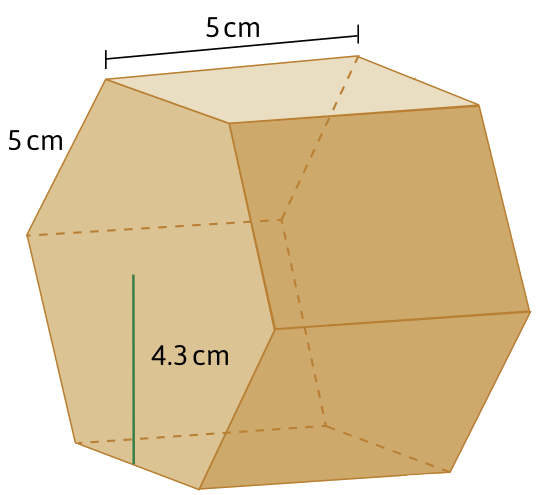
\includegraphics[width=.9\linewidth]{../images/20230319093449}
        \caption{}
        \label{fig:20230319093449}
    \end{figure}
\end{minipage}%
\begin{minipage}{0.65\linewidth}
    \begin{parts}
        \part Calcula su volumen

        \begin{solutionbox}{2cm}
            \[V=A_b h=\left(\dfrac{6\times 5 \text{ cm}\times 4.3 \text{ cm}}{2}\right)5 \text{ cm}=322.5 \text{ cm}^3
            \]
        \end{solutionbox}
        \part Otra caja de dulces tiene la misma forma, pero cada dimensión es el triple de las dimensiones de la otra caja. ¿Cuál será el volumen de esta segunda caja?

        \begin{solutionbox}{2.5cm}
            El volumen de una caja con el triple de dimensiones, sería:
            \[
                V=A_b h=\left(\dfrac{6\times 15 \text{ cm}\times 12.9 \text{ cm}}{2}\right)15 \text{ cm}= 8,707.5 \text{ cm}^3
            \]
        \end{solutionbox}
        \part ¿Cuántas veces es más grande el volumen de la caja mayor que la primera caja?

        \begin{solutionbox}{3cm}
            \[\dfrac{8,707.5 \text{ cm}^3}{322.5 \text{cm}^3}=27\]
            La caja con el triple de dimensiones es 27 veces mayor que la primera.
        \end{solutionbox}
    \end{parts}

\end{minipage}
